Located in one of the four intersections of the LHC beams, the CMS detector is designed to measure the resulting collisions to high precision. Key ingredients are a high precision measurements of the properties of single particles as well as a good coverage of the 4$\pi$ solid angle. The central element of the CMS detector is a superconducting solenoid. Cooled to $\unit{4.45}{\kelvin}$, it is able to produce a homogeneous magnetic field of $\unit{3.8}{\tesla}$, which allows to measure the momentum of charged particle by bending their trajectories. As shown in Figure~\ref{fig:CMS}, the different components of the detector are layered in cylindrical shapes around the interaction point. The magnet encompasses most of the main subdetectors, namely the tracking system which measures the trajectories of charged particles and the electromagnetic and hadron calorimeters, designed to measure the energy of particles. Located outside of the volume of the solenoid are the iron return yoke and muon detectors. This cylindrical structure is complemented on both sides by endcaps, which close the solid angle in the direction of the beams and are partly located outside the volume of the solenoid. The different components are described in more detail in the following. 
\begin{figure}[htbp]
\centering
  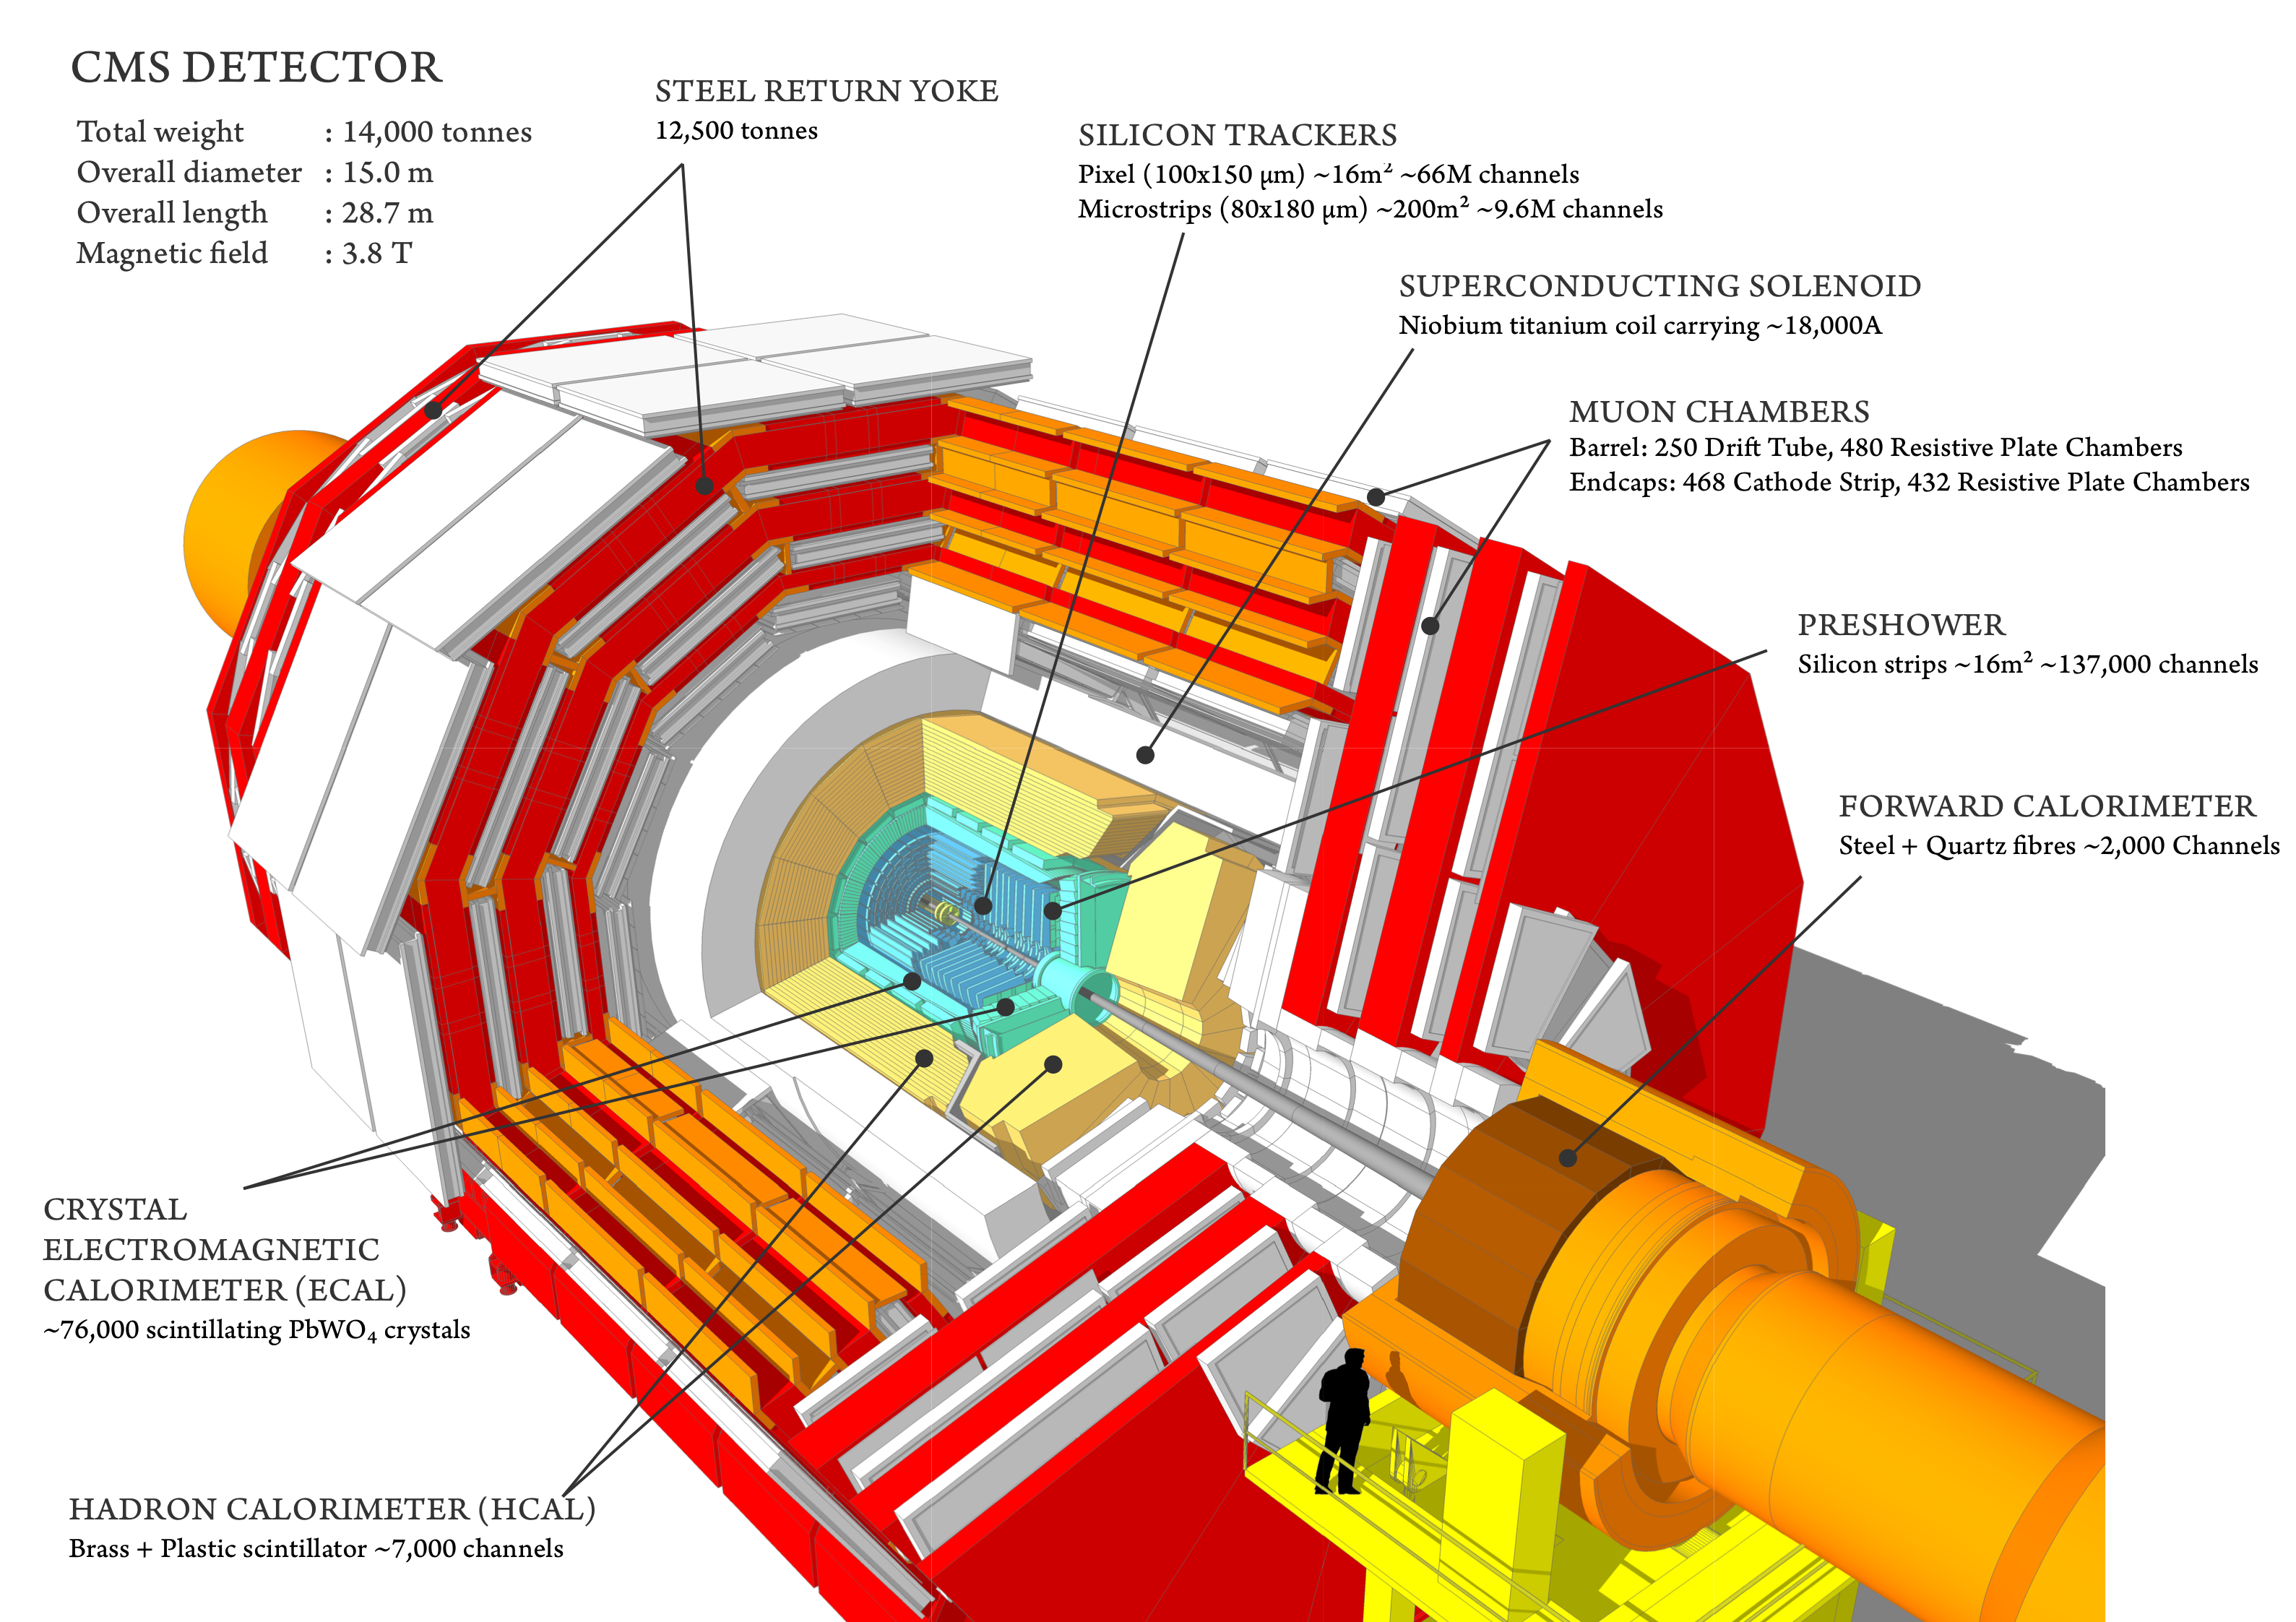
\includegraphics[width=0.6\textwidth]{plots/CMS/cms_design.png}
\caption{Schematic view of the CMS detector~\cite{CMSScetch}. From the inside out, the tracking system is shown in blue, the electromagnetic calorimeter in green, the hadron calorimeter in light yellow, the superconducting solenoid in white, the return yoke in red and the muon system again in white.}
\label{fig:CMS}
\end{figure}
\subsection{The tracking system}
The trajectory of charged particles can be determined by measuring the signal of the ionization they cause when traversing matter. The tracking system of the CMS detector consists of many layers of silicon pixels and strips. Combining the points at which a charged particle traverses the different layers, the trajectory of this particle can be measured. The bending of this trajectory under the influence of the magnetic field allows to determine the momentum of the particle. The tracking system has a diameter of $\unit{2.5}{\meter}$ and a length of $\unit{5.8}{\meter}$, corresponding to a geometric coverage of $\vert \eta \vert < $ 2.5. The tracking detector consists, as shown in Figure~\ref{fig:tracker}, of the pixel detector (PIXEL) surrounded by various components of  the silicon strip tracker. 
\begin{figure}[htbp]
\centering
  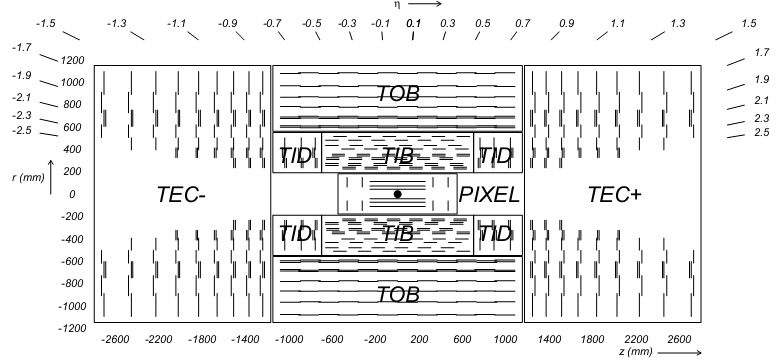
\includegraphics[width=0.6\textwidth]{plots/CMS/Tracker.png}
\caption{Schematic view of the CMS tracking detector. The innermost part shows the pixel detector (PIXEL), surrounded by the tracker inner barrel (TIB) and tracker inner discs (TID). The outermost parts of the tracking detector are the tracker outer barrel (TOB) and the two tracker endcaps (TEC+ and TEC-).}
\label{fig:tracker}
\end{figure} 
\subsubsection*{The silicon pixel detector}
The innermost part of the tracking system in the pixel detector, which consists of three layers in the barrel region at radii between $\unit{4.4}{\centi\meter}$ and $\unit{10.2}{\centi\meter}$, complemented by two discs perpendicular to the beam axis, located at $\vert z \vert = \unit{34.5}{\centi\meter}$ and  $\vert z \vert = \unit{46.5}{\centi\meter}$. As the particle density is highest close to the interaction point, a high granularity is needed to maintain a low occupancy of the pixel detector. Therefore the pixel detector consists of roughly 66 million pixels with a combined active area of about $\unit{1}{\meter\squared}$. Each pixel has a size of $\unit{150\times100}{\micro\meter\squared}$. The analogue readout of the pixels allows to combine the measurements of neighbouring pixels, bringing the spatial resolution down to 15 to $\unit{20}{\micro\meter}$. This is especially important for the reconstruction of the interaction vertices and the tagging of the secondary vertices from the decay of b-hadrons.
\subsubsection*{The silicon strip detector}
Further away from the interaction point, between $\unit{20}{\centi\meter}$ and $\unit{116}{\centi\meter}$, the granularity of the tracking system is reduced. Silicon strip detectors are used, structured in four layers of the tracker inner barrel (TIB), complemented on each side with three discs of the tracker inner discs (TID). All this is surrounded by the six layers of the tracker outer barrel (TOB). The tracker endcaps (TECs) consist of nine discs each. The individual strips have a length of about $\unit{10}{\centi\meter}$ and a pitch between $\unit{80}{\micro\meter}$ in the two inner layers of the TIB and $\unit{183}{\micro\meter}$ in the four inner layers of the TOB. The single point resolution in TIB and TOB depends on the layout of the specific layer and varies between $\unit{23}{\micro\meter}$ and $\unit{53}{\micro\meter}$. 

Stereo modules, constructed by placing two modules back to back, rotated by $\unit{100}{\milli\rad}$, are placed in the first two layers of both TIB and TOB, the first two discs of TID and the first two and the fifth discs of the TECs. These allow for 2-D measurements, with a precision of the $z$ position measurement of $\unit{230}{\micro\meter}$ in TIB and $\unit{530}{\micro\meter}$ in TOB. 

For high momentum tracks of about $\unit{100}{\giga\electronvolt}$ in the region of $\vert \eta \vert < 1.6$ a \pt resolution of 1-2\% is achieved, while the impact parameter of these tracks can be measured with a resolution of about $\unit{10}{\micro\meter}$. 

Compared to other tracking technologies, an all silicon tracking system as used in CMS consists of significantly more material. The material budget lies between 0.4 and 1.8 radiation length $X_0$, as shown in Figure~\ref{fig:trackerMaterial}. For light charged particles such as electrons this leads to a significant probability to emit bremsstrahlung in while traversing the tracking detector, which has to be taken into account in the reconstruction of particles.    
\begin{figure}[htbp]
\centering
  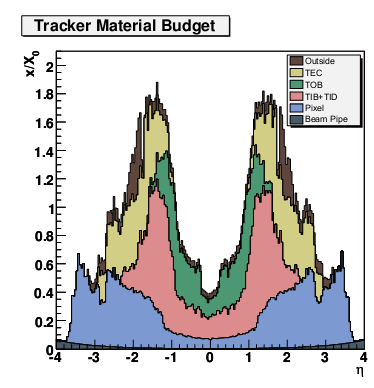
\includegraphics[width=0.6\textwidth]{plots/CMS/TrackerMaterial.png}
\caption{Material budget of the CMS tracking detector in units of radiation length $X_0$ as a function of $\eta$.}
\label{fig:trackerMaterial}
\end{figure} 
\subsection{The electromagnetic calorimeter}
The electromagnetic calorimeter (ECAL) measures the energy of electrons and photons. It uses lead tungstate ($PbWO_4$) crystals both as absorber and active material. The electromagnetic shower induced by the electron or photon leads to the emission of scintillation light in the crystal, which is measured at the end of the crystals by avalanche photo diodes (APDs) in the barrel segment of the ECAL and more radiation hard vacuum photo triods (VTPs) in the endcap region. The choice of lead tungstate was driven by the need for a material that is at the same time dense ($\unit{8.28}{\gram\per\centi\cubic\meter}$), has a small Molière radius ($\unit{2.2}{\centi\meter}$) and is fast. About 80\% of the scintillation light is emitted after $\unit{25}{\nano\second}$, which is the time between two LHC bunch crossing under design conditions. 
\begin{figure}[htbp]
\centering
  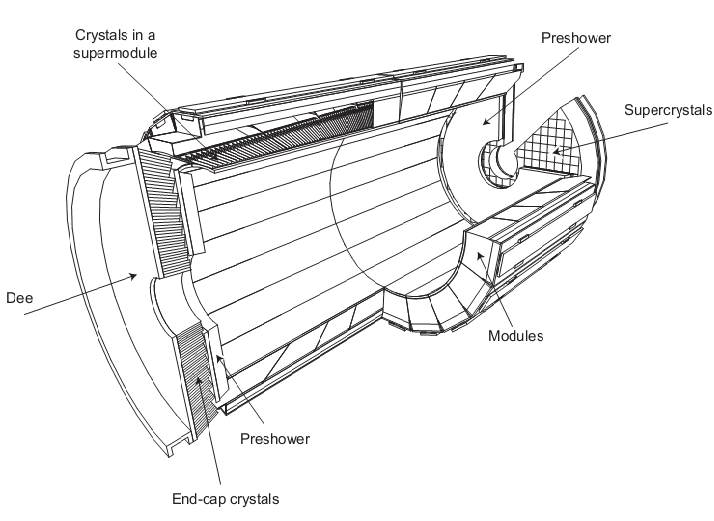
\includegraphics[width=0.6\textwidth]{plots/CMS/ECAL.png}
\caption{Schematic view of the CMS ECAL.}
\label{fig:ECAL}
\end{figure} 
The structure of the ECAL is shown in Figure~\ref{fig:ECAL}. The ECAL barrel (EB) covers the region of $\vert \eta \vert < 1.479$ and consists of 61200 crystals. They have a size of $\unit{2.2\times2.2}{\centi\meter\squared}$ at the front and $\unit{2.6\times2.6}{\centi\meter\squared}$ at the back, with a length of $\unit{23}{\centi\meter}$, corresponding to 25.8 $X_0$. In the ECAL endcaps (EE), consisting of 7324 crystal each, they are slightly larger ($\unit{2.862\times2.862}{\centi\meter\squared}$ to $\unit{3.0\times3.0}{\centi\meter\squared}$) and shorter ($\unit{22}{\centi\meter}$, corresponding to 24.7 $X_0$). The EEs extend the geometric coverage of the ECAL to $\vert \eta \vert = 3.0$. 

In the region of $1.653 < \vert \eta \vert < 2.6$ a preshower detector, consisting of two layers of silicon strips and two layers of lead absorber, is installed to distinguish between prompt photons and those from the decay $\pi^0 \rightarrow \gamma\gamma$. The strips, oriented perpendicular to each other, have a pitch of $\unit{2}{\milli\meter}$, allowing to resolve the two showers of the photons from the $\pi^0$. 

The production of scintillation photons per energy deposit is temperature depend. Therefore the ECAL is kept at a temperature of $\unit{18\pm0.05}{\celsius}$, where it is about 4.5 photons per MeV. 

The typical resolution of the ECAL is parametrized as
\begin{equation}
\left(\frac{\sigma}{E}\right)^2 = \left( \frac{2.8\%}{\sqrt{E}}\right)^2 + \left( \frac{0.12}{E} \right)^2 + (0.30\%)^2,
\end{equation}
with three terms describing different sources of uncertainty. The first term includes statistical fluctuation in the production of scintillation light as well as the energy distribution over several crystals. The second term covers such sources of noise as electronic noise or pileup. The constant term accounts for other sources of uncertainties such as calibration errors. The size of the different contributions has been confirmed in test beam measurements~\cite{EGM-10-003}. 
\subsection{The hadron calorimeter}

\subsection{The muon system} 